% -*- coding: utf-8 -*-
% Окружение как непосредственный связный список
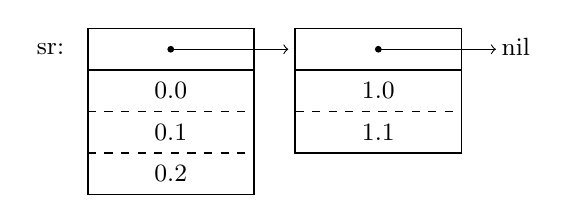
\begin{tikzpicture}
  \tikzstyle{every node}=[font=\small]

% список
  \draw (-0.5em, -0.75em) node[left] {\ic{sr}:};

  \draw [semithick] (0.0em, 0.0em) rectangle (6.0em, -6.0em);

  \filldraw  (3.0em, -0.75em) circle(1.0pt);
  \draw [->] (3.0em, -0.75em) -- (7.25em, -0.75em);

  \draw [semithick] (7.5em, 0.0em) rectangle (13.5em, -4.5em);

  \filldraw  (10.5em, -0.75em) circle(1.0pt);
  \draw [->] (10.5em, -0.75em) -- (14.75em, -0.75em);

  \draw (14.6em, -0.65em) node[right] {\ii{nil}};

% окружения
  \draw (0.0em, -1.5em) -- (6.0em, -1.5em);
  \draw          (3.0em, -1.6em) node[below] {\ic{0.0}};
  \draw [dashed] (0.0em, -3.0em) -- (6.0em, -3.0em);
  \draw          (3.0em, -3.1em) node[below] {\ic{0.1}};
  \draw [dashed] (0.0em, -4.5em) -- (6.0em, -4.5em);
  \draw          (3.0em, -4.6em) node[below] {\ic{0.2}};

  \draw (7.5em, -1.5em) -- (13.5em, -1.5em);
  \draw          (10.5em, -1.6em) node[below] {\ic{1.0}};
  \draw [dashed] ( 7.5em, -3.0em) -- (13.5em, -3.0em);
  \draw          (10.5em, -3.1em) node[below] {\ic{1.1}};

\end{tikzpicture}
